\subsection{Supercell}
All quantum Monte Carlo (QMC) calculations are performed using 72-atom simulation cells. Each simulation cell is tiled from the optimized unit cell using a supercell matrix.
\begin{align}
A_s = S A \Rightarrow \left(\begin{array}{c}
\bs{a}_s \\
\bs{b}_s \\
\bs{c}_s
\end{array}\right) = S\left(\begin{array}{c}
\bs{a} \\
\bs{b} \\
\bs{c}
\end{array}\right),
\end{align}
where $\bs{a}$, $\bs{b}$, $\bs{c}$ are the lattice vectors of the unit cell. $\bs{a}_s$, $\bs{b}_s$, $\bs{c}_s$ are the lattice vectors of the simulation cell. $S$ is the supercell matrix. The supercell matrices are chosen to maximize the simulation cell radius. %Ideally, one should maximize the image radius $R_{WS}$ instead.
\begin{table}[h]
\caption{Supercell matrices.}
\begin{tabular}{cccc}
\hline\hline
Cmca-4 & Cmca-12 & C2/c-24 & I4$_1$/amd \\
\hline
$\left(\begin{array}{ccc}
 3 &  3 &  0 \\
-1 &  2 &  1 \\
 2 & -1 &  1
\end{array}\right)$ & $\left(\begin{array}{ccc}
 2 &  1 &  -1 \\
-1 &  1 &  0 \\
 2 &  1 &  1
\end{array}\right)$ & $\left(\begin{array}{ccc}
 2 &  1 &  0 \\
 1 &  2 &  0 \\
 0 &  0 &  1
\end{array}\right)$ & $\left(\begin{array}{ccc}
 2 & -2 &  1 \\
 2 &  3 &  0 \\
-2 &  1 &  1
\end{array}\right)$ \\
\hline\hline
\end{tabular}
\end{table}

In Fig.~\ref{fig:cell-radius}, the image radius (a.k.a. radius of the real-space Wigner-Seitz cell) $R_{WS}$ and simulation cell radius $R_{sc}$ are shown as a function of density.

\begin{figure}[h]
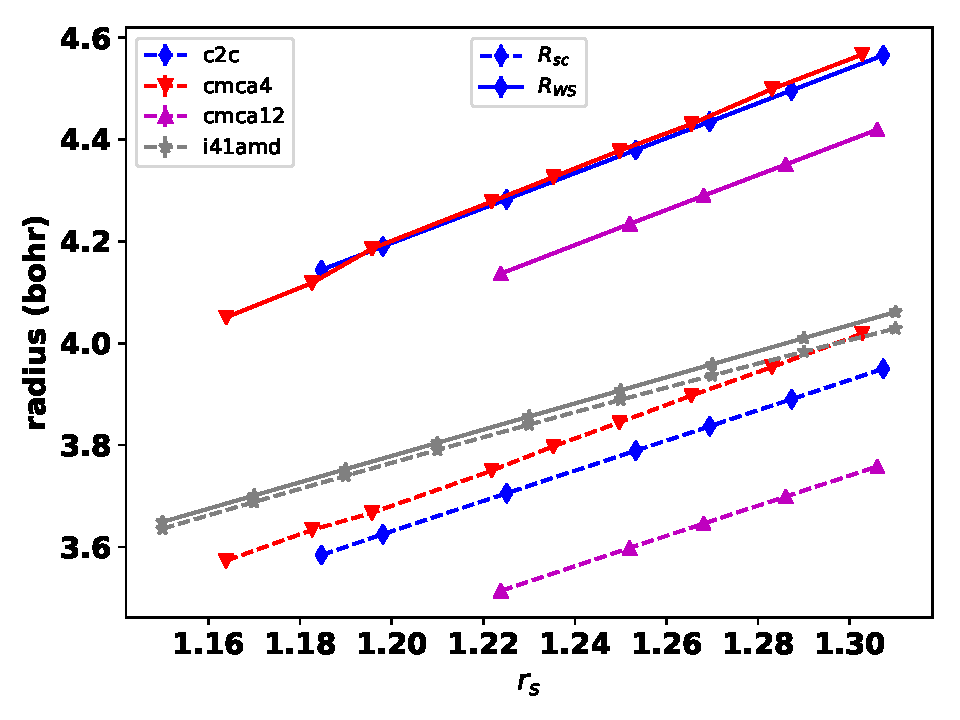
\includegraphics[width=0.8\columnwidth]{101a1_cell-radius}
\caption{Supercell radius as a function of density. $r_s$ is the Wigner-Seitz radius, which is determined by the average electron density $\frac{4\pi}{3}r_s=\rho$, where $\rho=N_e/\Omega$, with $\Omega$ the supercell volume. $R_{WS}$ is the radius of the real-space Wigner-Seitz cell of the supercell. $2R_{WS}$ is the minimum distance between periodic images. \label{fig:cell-radius}}
\end{figure}

\subsection{Wavefunction}

All QMC calculations are performed using the QMCPACK code. We use Slater-Jastrow-Backflow (SJB) wavefunction. The orbitals in the Slater determinant are cusp-corrected DFT orbitals. The vdw-DF functional is used to generate orbitals for the molecular structures, whereas the PBE functional is used for the atomic structure. The orbital generating DFT runs have different settings compared to the geometry optimization runs.

To generate the orbitals, we perform DFT directly in the supercell. All calculations use the bare Coulomb interaction and a plane wave cutoff of 50 Ry. First, we run a self-consistent calculation to converge the charge density on a shifted $8^3$ Monkhorst-Pack grid. Second, we run a non-self-consistent calculation on an unshifted Monkhorst-Pack grid to generate the orbitals needed by all twists. $4^3$ twists are used for the molecular phase, while $6^3$ twists are used for the atomic phase. Finally, we divide each orbital by an electron-ion Jastrow wavefunction to remove the electron-ion cusp from the orbital. This electron-ion Jastrow wavefunction is constructed using Fourier components commensurate with the simulation cell (i.e. on the reciprocal lattice vectors of the simulation cell $\bs{G}_s$)
\begin{align}
J_{ei}(\bs{r}_j; \bs{R}) \propto& \exp\left\{ \text{iFFT}\left[ 
U_{\bs{k}}^{ep}  \left(\sum\limits_{J=1}^{N_p} \frac{e^{-i\bs{k}\cdot\bs{R}_J}}{N_p}  \right)
\right] \right\} \nonumber\\
\propto& \exp\left\{ 
\sum\limits_{\bs{k}\neq\bs{0}}^{\bs{k}\in\bs{G}_s} e^{i\bs{k}\cdot\bs{r}_j}~
U_{\bs{k}}^{ep} 
\left(\sum\limits_{J=1}^{N_p} \frac{e^{-i\bs{k}\cdot\bs{R}_J}}{N_p}  \right)
\right\},\label{eq:rpa-ep-jas}
\end{align}
where $\bs{r}_j$ is any single electron coordinate. $\bs{R}$ contains all ionic coordinates. $N_p$ is the number of protons. iFFT stands for ``inverse fast Fourier transform''. The Jastrow potential $U_{\bs{k}}^{ep}$ in eq.~(\ref{eq:rpa-ep-jas}) is chosen to be the RPA form written by Ceperley and Alder
\begin{align}
2U^{ep}_k = -a_k(1+a_k)^{-1/2},
\end{align}
where $a_k=\frac{12}{r_s^3k^4}$ in Hartree atomic units. $r_s$ is the Wigner-Seitz radius.

When a single-particle orbital is divided by eq.~(\ref{eq:rpa-ep-jas}), the electron-ion cusp is removed from the orbital. We re-introduce the electron-ion cusp in the Jastrow part of the trial wavefunction. 

There are 48 optimizable parameters in our wavefunction. We use short-range B-spline Jastrow pair potentials which are smoothly cut off at $R_{WS}$ (the image radius). There are three Jastrow potentials (uu, ud, ep) between up and up electrons, up and down electrons, electron and proton. We use short-range B-spline back flow transformation functions which are smoothly cut off $R_{WS}$. There are three backflow correlation functions (uu, ud, ep) similar to the Jastrow setup. Each B-spline has 8 optimizable knots.

\subsection{QMC Data}

At each density, we perform one VMC and two DMC calculations. Each QMC calculation is labeled by a series index. The VMC calculation is series 0. The first DMC calculation with a relatively large time step is series 1. The second DMC calculation with a relatively small time step is series 2. We post-process the raw results (series 0 - 2) to produce series 3 and 4. We linearly extrapolate the DMC results (series 1, 2) to zero time step and label the results series 3. We linearly extrapolate the VMC and the t=0 DMC results (series 0, 3) to obtain pure-estimator kinetic and potential energies and label them series 4.

Twist-average QMC energies are displayed in the following table. The dUlr column contains the many-body finite size correction which will be described in the next section.

%\begin{table}[h]
%\small
%\begin{tabular}{llrrrllll}
\toprule
         &   &  timestep &  natom &      dUlr & LocalEnergy\_pp &    Variance\_pp &     Kinetic\_pp &    Potential\_pp \\
rs & series &           &        &           &                &                &                &                 \\
\midrule
1.163891 & 0 &    0.0300 &     72 &  0.005586 &    -0.47572(1) &     0.01380(2) &      0.9819(1) &      -1.4576(1) \\
         & 1 &    0.0030 &     72 &  0.005417 &   -0.477138(9) &    0.013719(9) &     0.98177(9) &     -1.45890(8) \\
         & 2 &    0.0015 &     72 &  0.005404 &    -0.47712(1) &     0.01374(1) &      0.9822(1) &    -1.45933(10) \\
         & 3 &    0.0000 &     72 &  0.005391 &    -0.47711(2) &     0.01374(1) &      0.9827(2) &      -1.4598(2) \\
         & 4 &    0.0000 &     72 &  0.005213 &    -0.47711(2) &     0.01374(1) &      0.9834(2) &      -1.4598(2) \\
1.182675 & 0 &    0.0300 &     72 &  0.005455 &    -0.48354(1) &     0.01347(2) &      0.9581(1) &      -1.4416(1) \\
         & 1 &    0.0030 &     72 &  0.005269 &   -0.484951(9) &    0.013408(8) &     0.95828(9) &     -1.44323(9) \\
         & 2 &    0.0015 &     72 &  0.005287 &    -0.48496(1) &     0.01342(1) &      0.9585(1) &      -1.4434(1) \\
         & 3 &    0.0000 &     72 &  0.005305 &    -0.48496(2) &     0.01342(1) &      0.9587(2) &      -1.4436(2) \\
         & 4 &    0.0000 &     72 &  0.005170 &    -0.48496(2) &     0.01342(1) &      0.9592(2) &      -1.4436(2) \\
1.195717 & 0 &    0.0300 &     72 &  0.005373 &   -0.488647(6) &    0.012795(9) &     0.94365(7) &     -1.43230(7) \\
         & 1 &    0.0030 &     72 &  0.005188 &   -0.490019(9) &    0.012688(8) &     0.94357(9) &     -1.43361(9) \\
         & 2 &    0.0015 &     72 &  0.005183 &   -0.490017(9) &    0.012707(9) &     0.94391(9) &     -1.43394(9) \\
         & 3 &    0.0000 &     72 &  0.005178 &    -0.49002(2) &    0.012707(9) &      0.9443(2) &      -1.4343(2) \\
         & 4 &    0.0000 &     72 &  0.004997 &    -0.49002(2) &    0.012707(9) &      0.9449(2) &      -1.4343(2) \\
1.221845 & 0 &    0.0300 &     72 &  0.005135 &   -0.497976(6) &    0.012288(9) &     0.91589(7) &     -1.41386(7) \\
         & 1 &    0.0030 &     72 &  0.004973 &   -0.499383(8) &    0.012232(9) &     0.91531(9) &     -1.41469(9) \\
         & 2 &    0.0015 &     72 &  0.004998 &   -0.499352(8) &    0.012255(9) &     0.91567(9) &     -1.41501(9) \\
         & 3 &    0.0000 &     72 &  0.005023 &    -0.49932(2) &    0.012255(9) &      0.9160(2) &      -1.4153(2) \\
         & 4 &    0.0000 &     72 &  0.004922 &    -0.49932(2) &    0.012255(9) &      0.9162(2) &      -1.4153(2) \\
1.235307 & 0 &    0.0300 &     72 &  0.005067 &   -0.502414(6) &     0.01188(1) &     0.90195(6) &     -1.40436(7) \\
         & 1 &    0.0030 &     72 &  0.004900 &   -0.503809(8) &    0.011814(8) &     0.90131(9) &     -1.40508(9) \\
         & 2 &    0.0015 &     72 &  0.004908 &   -0.503783(9) &    0.011793(9) &     0.90181(9) &     -1.40559(9) \\
         & 3 &    0.0000 &     72 &  0.004915 &    -0.50376(2) &    0.011793(9) &      0.9023(2) &      -1.4061(2) \\
         & 4 &    0.0000 &     72 &  0.004776 &    -0.50376(2) &    0.011793(9) &      0.9027(2) &      -1.4061(2) \\
1.249707 & 0 &    0.0300 &     72 &  0.004887 &   -0.506825(6) &     0.01274(2) &     0.88739(7) &     -1.39422(7) \\
         & 1 &    0.0030 &     72 &  0.004748 &   -0.508268(9) &    0.012682(9) &      0.8869(1) &     -1.39525(9) \\
         & 2 &    0.0015 &     72 &  0.004765 &   -0.508273(9) &    0.012696(9) &     0.88747(9) &     -1.39574(9) \\
         & 3 &    0.0000 &     72 &  0.004783 &    -0.50828(2) &    0.012696(9) &      0.8880(2) &      -1.3962(2) \\
         & 4 &    0.0000 &     72 &  0.004690 &    -0.50828(2) &    0.012696(9) &      0.8886(2) &      -1.3962(2) \\
1.265425 & 0 &    0.0300 &     72 &  0.004870 &   -0.511407(6) &     0.01158(1) &     0.87289(6) &     -1.38430(7) \\
         & 1 &    0.0030 &     72 &  0.004684 &   -0.512853(8) &    0.011519(8) &     0.87292(9) &     -1.38577(9) \\
         & 2 &    0.0015 &     72 &  0.004697 &   -0.512872(8) &    0.011541(8) &     0.87333(9) &     -1.38621(9) \\
         & 3 &    0.0000 &     72 &  0.004710 &    -0.51289(2) &    0.011541(8) &      0.8738(2) &      -1.3866(2) \\
         & 4 &    0.0000 &     72 &  0.004565 &    -0.51289(2) &    0.011541(8) &      0.8746(2) &      -1.3866(2) \\
1.283017 & 0 &    0.0300 &     72 &  0.004733 &   -0.516220(6) &    0.011305(9) &     0.85757(7) &     -1.37379(7) \\
         & 1 &    0.0030 &     72 &  0.004574 &   -0.517656(8) &    0.011240(9) &     0.85753(9) &     -1.37518(9) \\
         & 2 &    0.0015 &     72 &  0.004575 &   -0.517673(9) &    0.011251(8) &     0.85793(9) &     -1.37560(9) \\
         & 3 &    0.0000 &     72 &  0.004575 &    -0.51769(2) &    0.011251(8) &      0.8583(2) &      -1.3760(2) \\
         & 4 &    0.0000 &     72 &  0.004430 &    -0.51769(2) &    0.011251(8) &      0.8591(2) &      -1.3760(2) \\
1.302685 & 0 &    0.0300 &     72 &  0.004606 &   -0.521222(6) &    0.010863(8) &     0.84146(7) &     -1.36269(7) \\
         & 1 &    0.0030 &     72 &  0.004447 &   -0.522642(8) &    0.010795(7) &     0.84153(8) &     -1.36415(8) \\
         & 2 &    0.0015 &     72 &  0.004452 &   -0.522665(8) &    0.010810(8) &     0.84172(8) &     -1.36439(8) \\
         & 3 &    0.0000 &     72 &  0.004457 &    -0.52269(2) &    0.010810(8) &      0.8419(2) &      -1.3646(2) \\
         & 4 &    0.0000 &     72 &  0.004322 &    -0.52269(2) &    0.010810(8) &      0.8424(2) &      -1.3646(2) \\
\bottomrule
\end{tabular}

%\caption{Cmca-4}
%\end{table}
%
%\begin{table}[h]
%\small
%\begin{tabular}{llrrrllll}
\toprule
         &   &  timestep &  natom &      dUlr & LocalEnergy\_pp &     Variance\_pp &     Kinetic\_pp &   Potential\_pp \\
rs & series &           &        &           &                &                 &                &                \\
\midrule
1.223839 & 0 &    0.0300 &     72 &  0.005398 &   -0.498582(6) &     0.013259(9) &     0.91712(7) &    -1.41570(7) \\
         & 1 &    0.0030 &     72 &  0.005121 &   -0.500194(9) &     0.013059(9) &     0.91759(9) &    -1.41781(9) \\
         & 2 &    0.0015 &     72 &  0.005123 &   -0.500189(9) &     0.013063(9) &     0.91791(9) &    -1.41810(9) \\
         & 3 &    0.0000 &     72 &  0.005125 &    -0.50018(2) &     0.013063(9) &      0.9182(2) &     -1.4184(2) \\
         & 4 &    0.0000 &     72 &  0.004868 &    -0.50018(2) &     0.013063(9) &      0.9193(2) &     -1.4184(2) \\
1.251971 & 0 &    0.0300 &     72 &  0.005113 &   -0.507671(7) &     0.013093(9) &     0.89092(7) &    -1.39859(7) \\
         & 1 &    0.0030 &     72 &  0.004888 &   -0.509262(8) &     0.012973(9) &     0.89079(8) &    -1.40004(8) \\
         & 2 &    0.0015 &     72 &  0.004888 &   -0.509253(8) &     0.012967(9) &     0.89147(9) &    -1.40072(9) \\
         & 3 &    0.0000 &     72 &  0.004888 &    -0.50924(2) &     0.012967(9) &      0.8922(2) &     -1.4014(2) \\
         & 4 &    0.0000 &     72 &  0.004676 &    -0.50924(2) &     0.012967(9) &      0.8934(2) &     -1.4014(2) \\
1.268116 & 0 &    0.0300 &     72 &  0.005012 &   -0.512485(6) &     0.011951(8) &     0.87796(7) &    -1.39044(7) \\
         & 1 &    0.0030 &     72 &  0.004777 &   -0.514038(9) &     0.011822(9) &     0.87737(8) &    -1.39142(8) \\
         & 2 &    0.0015 &     72 &  0.004761 &   -0.514071(9) &     0.011820(9) &     0.87791(9) &    -1.39197(9) \\
         & 3 &    0.0000 &     72 &  0.004745 &    -0.51410(2) &     0.011820(9) &      0.8785(2) &     -1.3925(2) \\
         & 4 &    0.0000 &     72 &  0.004490 &    -0.51410(2) &     0.011820(9) &      0.8789(2) &     -1.3925(2) \\
1.286021 & 0 &    0.0300 &     72 &  0.004894 &    -0.51743(1) &      0.01155(1) &      0.8626(1) &     -1.3800(1) \\
         & 1 &    0.0030 &     72 &  0.004676 &   -0.518992(8) &     0.011411(9) &     0.86249(9) &    -1.38150(9) \\
         & 2 &    0.0015 &     72 &  0.004645 &    -0.51902(1) &    0.011398(10) &      0.8624(1) &     -1.3814(1) \\
         & 3 &    0.0000 &     72 &  0.004614 &    -0.51905(2) &    0.011398(10) &      0.8623(2) &     -1.3813(2) \\
         & 4 &    0.0000 &     72 &  0.004351 &    -0.51905(2) &    0.011398(10) &      0.8620(2) &     -1.3813(2) \\
1.306029 & 0 &    0.0300 &     72 &  0.004704 &   -0.522568(6) &      0.01157(2) &     0.84694(7) &    -1.36950(7) \\
         & 1 &    0.0030 &     72 &  0.004498 &   -0.524120(9) &     0.011457(9) &     0.84641(8) &    -1.37052(8) \\
         & 2 &    0.0015 &     72 &  0.004515 &   -0.524133(8) &     0.011450(8) &     0.84684(9) &    -1.37098(9) \\
         & 3 &    0.0000 &     72 &  0.004531 &    -0.52415(2) &     0.011450(8) &      0.8473(2) &     -1.3714(2) \\
         & 4 &    0.0000 &     72 &  0.004370 &    -0.52415(2) &     0.011450(8) &      0.8476(2) &     -1.3714(2) \\
\bottomrule
\end{tabular}

%\caption{Cmca-12}
%\end{table}
%
%\begin{table}[h]
%\small
%\begin{tabular}{llrrrllll}
\toprule
         &   &  timestep &  natom &      dUlr & LocalEnergy\_pp &     Variance\_pp &     Kinetic\_pp &   Potential\_pp \\
rs & series &           &        &           &                &                 &                &                \\
\midrule
1.184674 & 0 &    0.0300 &     72 &  0.005670 &    -0.48422(1) &      0.01254(2) &      0.9616(1) &     -1.4459(1) \\
         & 1 &    0.0030 &     72 &  0.005413 &   -0.485676(9) &    0.012399(10) &     0.96117(9) &    -1.44684(9) \\
         & 2 &    0.0015 &     72 &  0.005411 &    -0.48568(1) &    0.012389(10) &      0.9616(1) &     -1.4473(1) \\
         & 3 &    0.0000 &     72 &  0.005409 &    -0.48569(2) &    0.012389(10) &      0.9620(2) &     -1.4477(2) \\
         & 4 &    0.0000 &     72 &  0.005167 &    -0.48569(2) &    0.012389(10) &      0.9624(2) &     -1.4477(2) \\
1.198103 & 0 &    0.0300 &     72 &  0.005490 &    -0.48946(1) &      0.01307(2) &      0.9490(1) &     -1.4384(1) \\
         & 1 &    0.0030 &     72 &  0.005271 &   -0.490925(8) &     0.012934(9) &     0.94809(9) &    -1.43904(8) \\
         & 2 &    0.0015 &     72 &  0.005273 &    -0.49093(1) &      0.01295(1) &      0.9487(1) &     -1.4396(1) \\
         & 3 &    0.0000 &     72 &  0.005275 &    -0.49093(2) &      0.01295(1) &      0.9493(2) &     -1.4402(2) \\
         & 4 &    0.0000 &     72 &  0.005080 &    -0.49093(2) &      0.01295(1) &      0.9496(2) &     -1.4402(2) \\
1.225107 & 0 &    0.0300 &     72 &  0.005412 &   -0.499215(7) &     0.011982(8) &     0.92039(7) &    -1.41960(7) \\
         & 1 &    0.0030 &     72 &  0.005135 &   -0.500680(9) &     0.011825(8) &     0.91983(9) &    -1.42051(9) \\
         & 2 &    0.0015 &     72 &  0.005138 &   -0.500694(9) &     0.011830(8) &     0.92029(9) &    -1.42099(9) \\
         & 3 &    0.0000 &     72 &  0.005140 &    -0.50071(2) &     0.011830(8) &      0.9207(2) &     -1.4215(2) \\
         & 4 &    0.0000 &     72 &  0.004886 &    -0.50071(2) &     0.011830(8) &      0.9211(2) &     -1.4215(2) \\
1.253286 & 0 &    0.0300 &     72 &  0.005220 &   -0.508316(6) &      0.01170(1) &     0.89260(7) &    -1.40092(7) \\
         & 1 &    0.0030 &     72 &  0.004942 &   -0.509765(9) &      0.01152(1) &     0.89257(8) &    -1.40232(8) \\
         & 2 &    0.0015 &     72 &  0.004929 &   -0.509798(8) &     0.011498(8) &      0.8929(1) &    -1.40282(9) \\
         & 3 &    0.0000 &     72 &  0.004917 &    -0.50983(2) &     0.011498(8) &      0.8933(2) &     -1.4033(2) \\
         & 4 &    0.0000 &     72 &  0.004634 &    -0.50983(2) &     0.011498(8) &      0.8940(2) &     -1.4033(2) \\
1.269426 & 0 &    0.0300 &     72 &  0.005052 &   -0.513065(6) &     0.011097(9) &     0.87708(7) &    -1.39014(7) \\
         & 1 &    0.0030 &     72 &  0.004806 &   -0.514529(8) &     0.010948(8) &     0.87756(9) &    -1.39209(9) \\
         & 2 &    0.0015 &     72 &  0.004799 &   -0.514517(8) &     0.010939(8) &     0.87786(9) &    -1.39238(9) \\
         & 3 &    0.0000 &     72 &  0.004792 &    -0.51451(2) &     0.010939(8) &      0.8782(2) &     -1.3927(2) \\
         & 4 &    0.0000 &     72 &  0.004549 &    -0.51451(2) &     0.010939(8) &      0.8792(2) &     -1.3927(2) \\
1.287311 & 0 &    0.0300 &     72 &  0.004946 &   -0.518053(6) &     0.010534(8) &     0.86353(7) &    -1.38158(7) \\
         & 1 &    0.0030 &     72 &  0.004690 &   -0.519484(9) &     0.010371(8) &     0.86319(9) &    -1.38267(9) \\
         & 2 &    0.0015 &     72 &  0.004683 &   -0.519499(9) &     0.010369(7) &     0.86374(8) &    -1.38325(9) \\
         & 3 &    0.0000 &     72 &  0.004675 &    -0.51951(2) &     0.010369(7) &      0.8643(2) &     -1.3838(2) \\
         & 4 &    0.0000 &     72 &  0.004423 &    -0.51951(2) &     0.010369(7) &      0.8651(2) &     -1.3838(2) \\
1.307314 & 0 &    0.0300 &     72 &  0.004801 &    -0.52318(1) &      0.01054(2) &      0.8471(1) &     -1.3703(1) \\
         & 1 &    0.0030 &     72 &  0.004552 &   -0.524617(8) &     0.010398(8) &     0.84732(9) &    -1.37196(9) \\
         & 2 &    0.0015 &     72 &  0.004552 &    -0.52464(1) &      0.01039(1) &      0.8478(1) &     -1.3724(1) \\
         & 3 &    0.0000 &     72 &  0.004552 &    -0.52466(2) &      0.01039(1) &      0.8483(2) &     -1.3729(2) \\
         & 4 &    0.0000 &     72 &  0.004322 &    -0.52466(2) &      0.01039(1) &      0.8494(2) &     -1.3729(2) \\
\bottomrule
\end{tabular}

%\caption{C2/c-24}
%\end{table}
%
%\begin{table}[h]
%\small
%\begin{tabular}{llrrrllll}
\toprule
     &   &  timestep &  natom &      dUlr &  LocalEnergy\_pp &     Variance\_pp &      Kinetic\_pp &   Potential\_pp \\
rs & series &           &        &           &                 &                 &                 &                \\
\midrule
1.15 & 0 &    0.0300 &     72 &  0.006282 &    -0.468339(9) &      0.02039(2) &      0.97451(7) &    -1.44285(7) \\
     & 1 &    0.0030 &     72 &  0.005793 &     -0.47074(1) &      0.01978(1) &      0.97496(9) &    -1.44572(9) \\
     & 2 &    0.0015 &     72 &  0.005797 &     -0.47073(1) &      0.01980(1) &      0.97534(9) &    -1.44607(9) \\
     & 3 &    0.0000 &     72 &  0.005800 &     -0.47072(3) &      0.01980(1) &       0.9757(2) &     -1.4464(2) \\
     & 4 &    0.0000 &     72 &  0.005371 &     -0.47072(3) &      0.01980(1) &       0.9769(2) &     -1.4464(2) \\
1.17 & 0 &    0.0300 &     72 &  0.006168 &    -0.476700(9) &      0.02044(2) &      0.94912(7) &    -1.42582(8) \\
     & 1 &    0.0030 &     72 &  0.005678 &    -0.479108(9) &      0.01981(1) &      0.94928(7) &    -1.42839(7) \\
     & 2 &    0.0015 &     72 &  0.005659 &    -0.479149(9) &      0.01981(1) &      0.94962(7) &    -1.42876(7) \\
     & 3 &    0.0000 &     72 &  0.005639 &     -0.47919(2) &      0.01981(1) &       0.9499(2) &     -1.4291(2) \\
     & 4 &    0.0000 &     72 &  0.005158 &     -0.47919(2) &      0.01981(1) &       0.9508(2) &     -1.4291(2) \\
1.19 & 0 &    0.0300 &     72 &  0.005965 &   -0.484386(10) &      0.02117(2) &      0.92299(7) &    -1.40738(7) \\
     & 1 &    0.0030 &     72 &  0.005520 &     -0.48679(1) &      0.02062(2) &      0.92317(9) &    -1.40994(9) \\
     & 2 &    0.0015 &     72 &  0.005508 &     -0.48683(1) &      0.02062(2) &      0.92352(9) &    -1.41035(9) \\
     & 3 &    0.0000 &     72 &  0.005497 &     -0.48687(3) &      0.02062(2) &       0.9239(2) &     -1.4108(2) \\
     & 4 &    0.0000 &     72 &  0.005077 &     -0.48687(3) &      0.02062(2) &       0.9248(2) &     -1.4108(2) \\
1.21 & 0 &    0.0300 &     72 &  0.005837 &     -0.49145(1) &       0.0197(2) &       0.9000(1) &     -1.3914(1) \\
     & 1 &    0.0030 &     72 &  0.005390 &   -0.493853(10) &      0.01908(1) &      0.89966(7) &    -1.39351(7) \\
     & 2 &    0.0015 &     72 &  0.005394 &   -0.493893(10) &      0.01908(1) &      0.89987(7) &    -1.39376(7) \\
     & 3 &    0.0000 &     72 &  0.005398 &     -0.49393(2) &      0.01908(1) &       0.9001(2) &     -1.3940(2) \\
     & 4 &    0.0000 &     72 &  0.005002 &     -0.49393(2) &      0.01908(1) &       0.9002(2) &     -1.3940(2) \\
1.23 & 0 &    0.0300 &     72 &  0.005709 &     -0.49788(1) &      0.01952(6) &       0.8772(1) &     -1.3751(1) \\
     & 1 &    0.0030 &     72 &  0.005260 &    -0.500351(9) &      0.01906(1) &      0.87668(7) &    -1.37703(7) \\
     & 2 &    0.0015 &     72 &  0.005243 &    -0.500363(9) &      0.01905(1) &      0.87711(7) &    -1.37748(7) \\
     & 3 &    0.0000 &     72 &  0.005226 &     -0.50038(2) &      0.01905(1) &       0.8775(2) &     -1.3779(2) \\
     & 4 &    0.0000 &     72 &  0.004781 &     -0.50038(2) &      0.01905(1) &       0.8779(2) &     -1.3779(2) \\
1.25 & 0 &    0.0300 &     72 &  0.005701 &     -0.50380(1) &      0.01725(2) &       0.8546(1) &     -1.3584(1) \\
     & 1 &    0.0030 &     72 &  0.005192 &    -0.506311(9) &    0.016644(10) &      0.85476(7) &    -1.36107(7) \\
     & 2 &    0.0015 &     72 &  0.005195 &    -0.506295(9) &    0.016635(10) &      0.85502(7) &    -1.36131(7) \\
     & 3 &    0.0000 &     72 &  0.005199 &     -0.50628(2) &    0.016635(10) &       0.8553(2) &     -1.3615(2) \\
     & 4 &    0.0000 &     72 &  0.004741 &     -0.50628(2) &    0.016635(10) &       0.8560(2) &     -1.3615(2) \\
1.27 & 0 &    0.0300 &     72 &  0.005504 &     -0.50918(1) &      0.01858(2) &       0.8365(1) &     -1.3457(1) \\
     & 1 &    0.0030 &     72 &  0.005037 &    -0.511700(9) &      0.01807(1) &      0.83566(7) &    -1.34736(7) \\
     & 2 &    0.0015 &     72 &  0.005031 &   -0.511705(10) &      0.01808(1) &      0.83584(7) &    -1.34755(7) \\
     & 3 &    0.0000 &     72 &  0.005025 &     -0.51171(2) &      0.01808(1) &       0.8360(2) &     -1.3477(2) \\
     & 4 &    0.0000 &     72 &  0.004588 &     -0.51171(2) &      0.01808(1) &       0.8355(2) &     -1.3477(2) \\
1.29 & 0 &    0.0300 &     72 &  0.005491 &     -0.51409(1) &      0.01634(2) &     0.81539(10) &     -1.3295(1) \\
     & 1 &    0.0030 &     72 &  0.004980 &   -0.516579(10) &      0.01577(1) &      0.81540(7) &    -1.33198(7) \\
     & 2 &    0.0015 &     72 &  0.004968 &    -0.516601(9) &      0.01579(1) &      0.81556(7) &    -1.33216(7) \\
     & 3 &    0.0000 &     72 &  0.004955 &     -0.51662(2) &      0.01579(1) &       0.8157(2) &     -1.3323(2) \\
     & 4 &    0.0000 &     72 &  0.004467 &     -0.51662(2) &      0.01579(1) &       0.8160(2) &     -1.3323(2) \\
1.31 & 0 &    0.0300 &     72 &  0.005418 &     -0.51851(1) &      0.01569(2) &       0.7983(1) &     -1.3168(1) \\
     & 1 &    0.0030 &     72 &  0.004889 &    -0.521027(9) &    0.015035(10) &      0.79760(7) &    -1.31862(7) \\
     & 2 &    0.0015 &     72 &  0.004880 &    -0.521046(9) &     0.015035(9) &      0.79801(7) &    -1.31906(7) \\
     & 3 &    0.0000 &     72 &  0.004871 &     -0.52106(2) &     0.015035(9) &       0.7984(2) &     -1.3195(2) \\
     & 4 &    0.0000 &     72 &  0.004371 &     -0.52106(2) &     0.015035(9) &       0.7985(2) &     -1.3195(2) \\
\bottomrule
\end{tabular}

%\caption{I4$_1$/amd}
%\end{table}

\subsection{Many-body Finite Size Correction}

We use the fluctuating structure factor $\delta S(\bs{k})\equiv \braket{(\rho_{\bs{k}}-\bar{\rho}_{\bs{k}})(\rho_{-\bs{k}}-\bar{\rho}_{-\bs{k}})}$ to calculate many-body finite size correction (FSC) to the potential energy. The integrand is cut off using optimized long-range Coulomb potential in reciprocal space $v_k^{lr}$
\begin{align}
\Delta V^{lr} = \left[\int - \sum\right] \frac{1}{2}v^{lr}_k \delta S(\bs{k}).
\end{align}
Total energy FSC ($\Delta E$) is a sum of kinetic ($\Delta T$) and potential ($\Delta V$) corrections regardless of whether mixed-estimator (m) or pure-estimator (p) is used
\begin{align}
\Delta E = \Delta T_m + \Delta V_m = \Delta T_p + \Delta V_p.
\end{align}
Without long-range wavefunction components, the mixed-estimator kinetic FSC is approximately zero ($\Delta T_m \approx 0$). Therefore
\begin{align}
\left\{\begin{array}{l}
\Delta E \approx \Delta V_m \\
\Delta T_p \approx \Delta V_m - \Delta V_p
\end{array}\right..
\end{align}
FSC of the Virial pressure ($\Delta P$) is then
\begin{align}
\left\{\begin{array}{l}
\Delta P_m = (2\Delta T_m + \Delta V_m)/(3\Omega) \approx (\Delta V_m)/(3\Omega) \\
\Delta P_p = (2\Delta T_p + \Delta V_p)/(3\Omega) \approx (2\Delta V_m-\Delta V_p)/(3\Omega)
\end{array}\right., \label{eq:pm-pp-fsc}
\end{align}
where $\Omega$ is volume. Regardless of whether mix-estimator or pure-estimator value is used for the Virial pressure, the FSC DMC enthalpy-pressure data agree well with equation of state derived from the total energy (Fig.~\ref{fig:si-static-hp}).

\subsection{Finite Size Corrected Data}

\begin{figure}[h]
\begin{minipage}{0.48\textwidth}
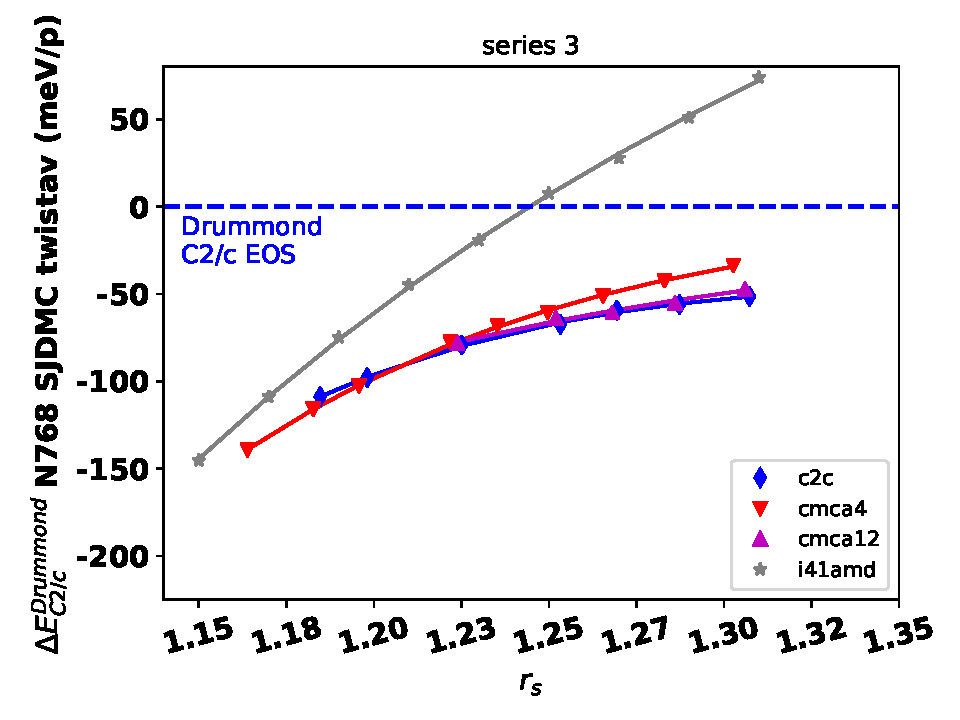
\includegraphics[width=0.8\columnwidth]{101sd_ev-s3}
%\caption{Energy v.s. volume.\label{fig:si-static-ev}}
\end{minipage}
\begin{minipage}{0.48\textwidth}
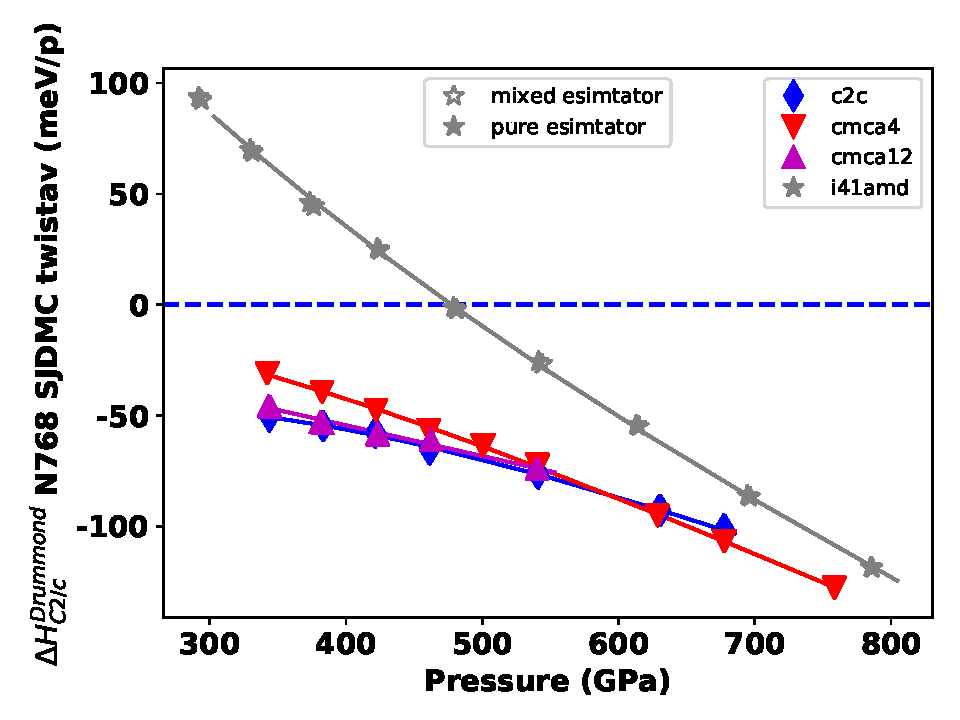
\includegraphics[width=0.8\columnwidth]{101se_hp}
%\caption{Enthalpy v.s. pressure.\label{fig:si-static-hp}}
\end{minipage}
\caption{Static-lattice DMC equation-of-state (EOS) relative to Drummond reference $E(\nu) = \frac{2.14020118}{\nu^2} + \frac{0.60521235}{\nu} - 0.6073132$, where $\nu$ is volume per proton in bohr$^3$ and $E(\nu)$ is in Hartree atomic unit. Relative energies are shown in meV per proton (meV/p). Each solid line is obtained using a fitted energy-volume EOS. The EOS is obtained by fitting the finite-size corrected (FSC) total energy as a quadratic function of inverse volume. The markers are finite-size corrected simulation data without performing a fit. \label{fig:static-qmc-vs-drummond}}
\end{figure}

\begin{comment}
Finally, we divide each orbital by an electron-ion Jastrow constructed on the reciprocal lattice vectors of the simulation cell $\bs{G}_s$
\begin{align}
J_{ei}(\bs{r}; \bs{R}) = \exp\left\{ -\frac{1}{2\Omega} \sum\limits_{\bs{k}\neq\bs{0}}^{\bs{k}\in\bs{G}_s}
U_{\bs{k}}^{ei} 
\left(\frac{1}{N}\sum\limits_{j=1}^{N_e} e^{i\bs{k}\cdot\bs{r}_j} \right)
\left(\frac{1}{N}\sum\limits_{J=1}^{N_p} e^{-i\bs{k}\cdot\bs{R}_J}  \right)
\right\},\label{eq:rpa-ep-jas}
\end{align}
\begin{align}
J_{ei}(\bs{r}_j; \bs{R}) =& \exp\left\{ \text{iFFT}\left[ 
U_{\bs{k}}^{ep}  \left(\sum\limits_{J=1}^{N_p} \frac{e^{-i\bs{k}\cdot\bs{R}_J}}{N_p}  \right)
\right] \right\}\\
=& \exp\left\{ 
-\frac{(2\pi)^3}{\Omega N_k} \sum\limits_{\bs{k}\neq\bs{0}}^{\bs{k}\in\bs{G}_s} e^{i\bs{k}\cdot\bs{r}_j}~
U_{\bs{k}}^{ep} 
\left(\sum\limits_{J=1}^{N_p} \frac{e^{-i\bs{k}\cdot\bs{R}_J}}{N_p}  \right)
\right\},\label{eq:rpa-ep-jas}
\end{align}
where $\Omega$ is the simulation cell volume. $\bs{r}$ contain all electronic coordinates, $\bs{R}$ contain all ionic coordinates. $N_e$ is the number of electrons, while $N_p$ is the number of protons.
The Jastrow potential $U_{\bs{k}}^{ei}$ in eq.~(\ref{eq:rpa-ep-jas}) is chosen to be the RPA form written by Ceperley and Alder
\begin{align}
2U^{ei}_k = -a_k(1+a_k)^{-1/2},
\end{align}
where $a_k=\frac{12}{r_s^3k^4}$ in Hartree atomic units.
\end{comment}